\documentclass{article}
\usepackage[utf8]{inputenc}
\usepackage{graphicx}


\begin{document}
\subsection{Natural Logarithm of 2}
\noindent
\begin{itemize}
    \item The natural log gives you the time needed to reach a certain level of growth.
    \item The natural log is the inverse of e, the Latin name is logarithmus naturali, giving the abbreviation $\ln()$.
    \item $\ln(1)$ = 0; which means that there is no time growth from 1 to 1.
    \item $\ln(0.5)$ = undefined; because we can not have a negative time progress.
    \item $\ln(negative number)$ = undefined; Undefined just means “there is no amount of time you can wait” to get a negative amount.
    \item The natural log can be used with any interest rate or time as long as their product is the same.
\end{itemize}
\textbf{Algebric Number:} To be algebraic, a number must be a root of a non-zero polynomial equation with rational coefficients.\\
\textbf{Transcendental Number:} A Transcendental Number is any number that is not an Algebraic Number.\\
The natural logarithm of 2 is a transcendental quantity.
\\textbf{$\ln(2)$} = 0.6931472.. \\
It is not known if $\ln(2)$ is normal.\\ 
$\sum_1^\infty{\frac{(-1)^{k+1}}{k}} = \ln(2) = 0.693..$
\begin{figure}[h!]
    \centering
    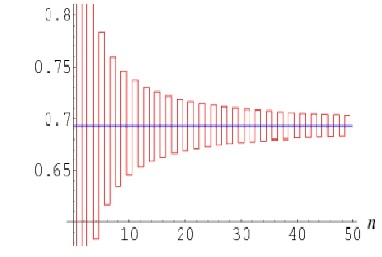
\includegraphics{Natural_Log_Of_2.jpg}
\end{figure}
\\
\textbf{Question: How long to double the money at 100\% interest?} \\
Answer: $\ln(2)$ = .693. It takes .693 units of time to double your money with continuous compounding with a rate of 100%.
\end{document}